\section{Analysis}
In this section, we analyse the datasets and present some general statistics and trends from the datasets described in the previous section.

\subsection{RfA statistics}
In Figure~\ref{fig:Election-stats}, we see statistics of elections in Wikipedia that show some interesting trends. First, in Figure~\ref{fig:vot-distribution} we see that the average number of votes in elections is increasing with time. This is expected, as initial RfA were just confirmation processes for candidates who were qualified. As the years went by the process starts to get more involved. This is seen in Figure~\ref{fig:num-rfas}, where there is a peak in the number of successful and unsuccessful elections around 2008 and since then there are fewer election and in total fewer successful ones. A pattern to note: the distribution of votes show that there is a clear majority of support votes in Figure~\ref{fig:vote-type-distribution}. An interesting fact is that the average number of words in comments seen in Figure~\ref{fig:comment-distribution} show that support votes have much fewer words compared to oppose or neutral votes. This indicates that people who are casting support votes might have small positive comments, while people casting negative or neutral votes tend to write larger comments to convince others of the issues that they find in the candidacy.

\subsection{Influential Voters}
\label{sec:influential-voters}
To find if there is a set of voters in elections who are influential, we utilized two approaches. The first is performing feature selection using a gradient boosting model on the whole dataset as done by Desai et al.\ \cite{desai2014result}. The second approach is similar to finding a set cover.

For the first approach, we created a dataset where each row corresponds to an election and each column is one user. Therefore as we have 4\,548 elections and nearly 13\,000 users so the data matrix is $X\in \mathbb{R}^{4548\times 13000}$ and the target is the result of the election, therefore $y_i\in \{1,-1\}$ and $y\in \mathbb{R}^{4548}$. Most users don not vote in all elections; therefore, the data matrix is very sparse. Unlike Desai et al.\ \cite{desai2014result}, we did not fill the unknown votes with 0s, instead we left them as missing values. This is because the XGBoost model is able to handle missing values. After fitting the model with the data we extracted the top 15 features based the \textit{gain} they bring to the model and is shown in Figure~\ref{fig:xgboost-feat-importance}. 
% These top 15 users can be thought of as the most influential voters for predicting an election.
\begin{figure}[!ht]
    \centering
    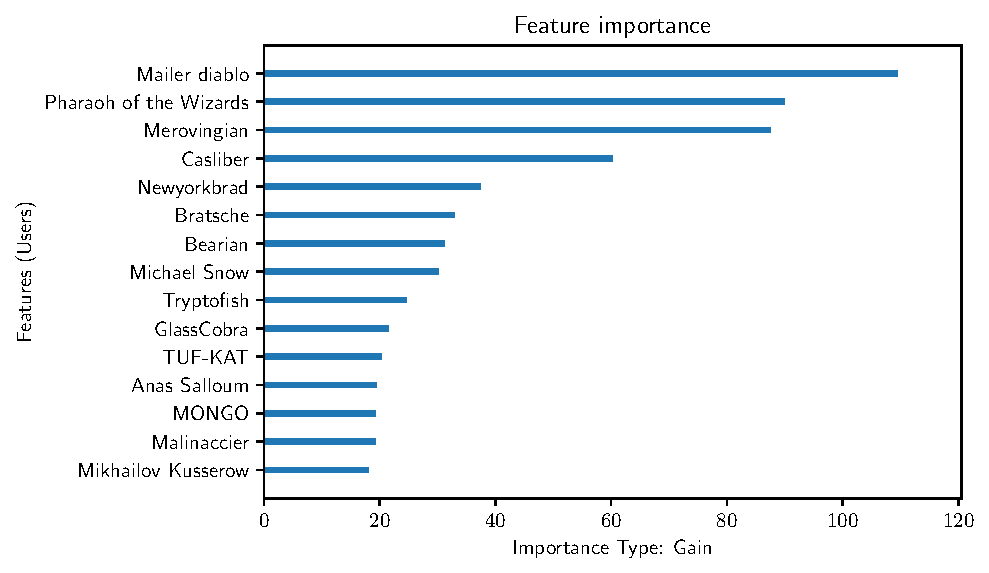
\includegraphics[width=\linewidth]{images/xgboost_features.pdf}
    \caption{XGBoost feature importance}
    \label{fig:xgboost-feat-importance}
\end{figure}

The second approach was formulating a set cover problem, every element of the ground set is a tuple of $(\text{voter},\text{election})$ and then we create a subset for each unique user. For every user we take each election they participated in and add the people who \textit{follow} that user. A user $u$ is said to follow the user $v$ if $u$ voted after $v$ they and they both voted the same. Therefore the set $S_u$ for every user is defined as 
\[
    S_{u} = \{(v,e) \mid \text{where } v \text{ voted the same after } u \text{ in election }e  \} 
\]
Then we order the subsets $S_u$ by their size and then try to find how much of the ground set we can cover by taking the top $k$ users' subsets. The ground set has $221\,766$ elements, which is fewer than the total number of votes as there are certain elections where either votes were duplicated or people voted twice. Now, we see how the set cover increases as we increase the value of $k$ as shown in Figure~\ref{fig:set-cover}.
\begin{figure}[!ht]
    \centering
    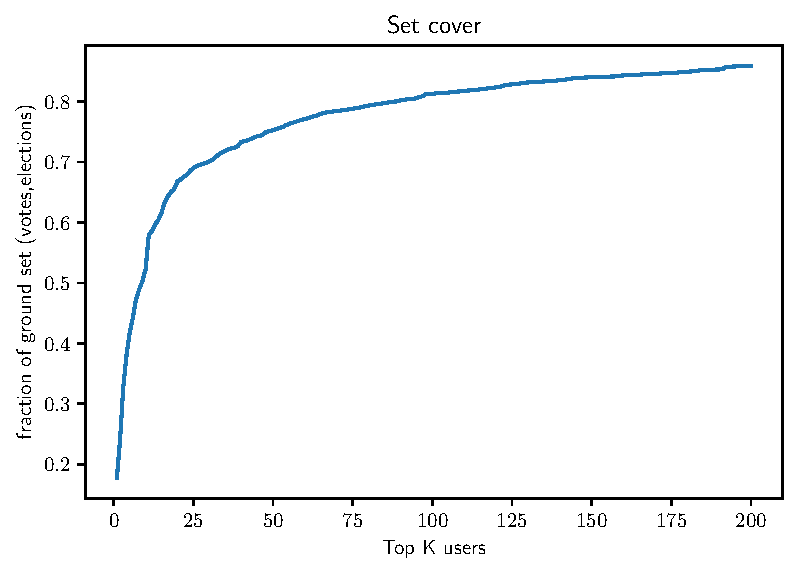
\includegraphics[width=\linewidth]{images/set_cover.pdf}
    \caption{Election set cover}
    \label{fig:set-cover}
\end{figure}
We see that with the top $200$ users we cover nearly $85\%$ of the whole ground set. With the top $15$ users we have $60\%$ coverage. More interestingly, we see that there is a knee around top 25 users and a set cover of $70\%$ indicating that there is a small core of influential users.  

\begin{table}[!ht]
    \centering
    \caption{Top 10 influential users from XGBoost and the Set Cover models}
    \label{tab:top-10}
    \begin{tabular}{clr}
        \toprule
        Ranking&XGBoost&Set Cover\\
        \midrule
        1& Mailer diablo & Siva1979\\
        2&Pharaoh of the Wizards&Mailer diablo\\
        3&Merovingian&Newyorkbrad\\
        4&Casliber&Wizardman\\
        5&Newyorkbrad&Pedro\\
        6&Bratsche&Dlohcierekim\\
        7&Bearian&Juliancolton\\
        8&Michael Snow&Casliber\\
        9&Tryptofish&Acalamari\\
        10&GlassCobra&Fastily\\
        \bottomrule
    \end{tabular}
\end{table}
In Table~\ref{tab:top-10} we see many common users among the top 10 influential users from both approaches. This confirms the fact that in Wikipedia RfA elections there is a core set of voters who can be important in predicting the result of an election.